%+----------------------------------------------------------------------------+
%| SLIDES: Constraint Algebras of multisymplectic Observables (Follow-up talk)
%| Contents:	- 25 minutes (extimated duration ~2 minutes per slide, ~12 slides )
%|
%| Author: Antonio miti
%| Event: 19th International Young Researchers Workshop on Geometry, Dynamics and Field Theory
%| Place: Verona
%| Date: 20/01/25
%+----------------------------------------------------------------------------+


%- HandOut Flag -----------------------------------------------------------------------------------------
	\newif\ifHandout
	\Handouttrue  %uncomment for the printable version
	%Handling of flags it is not preserved when passing to standalone-subfiles!


%- D0cum3nt ----------------------------------------------------------------------------------------------
\ifHandout
	\documentclass[handout,10pt]{beamer}   
	\setbeameroption{show notes} %print notes   
\else
	\documentclass[10pt]{beamer}
\fi


%- Packages ----------------------------------------------------------------------------------------------
\usepackage{custom-style}
\usepackage{math}

%- Bibliography (Biber) ----------------------------------------------------------------------------------
\usepackage[backend=biber,style=alphabetic,maxnames=2]{biblatex}
\bibliography{bibfile.bib}

%- L30's ----------------------------------------------------------------------------------------------
\usepackage{quiver} %https://q.uiver.app/ % Not in Miktex!
\usetikzlibrary{nfold}
\usetikzlibrary{decorations.pathmorphing} 
\renewcommand{\Ham}{\mathrm{Ham}}
\renewcommand{\Der}{\mathrm{Der}}
\usepackage{enumitem}
\setlist{topsep=0pt, leftmargin=*,label=$\bullet$}


%--Beamer Style-----------------------------------------------------------------------------------------------
\usetheme{toninus}

\usetikzlibrary{backgrounds}
  \tikzset{
    invisible/.style={opacity=0},
    visible on/.style={alt=#1{}{invisible}},
    alt/.code args={<#1>#2#3}{%
      \alt<#1>{\pgfkeysalso{#2}}{\pgfkeysalso{#3}} % \pgfkeysalso doesn't change the path
    },
  }


%- T1tle P4g3 -------------------------------------------------------------------------------------------
\title{ Constraint Algebras \\ of Multisymplectic Observables } 
\subtitle{\href{https://sites.google.com/view/xix-yrw-verona/home?authuser=0}{19th International Young Researchers Workshop on Geometry, Dynamics and Field Theory}}
\author[AMM]{
	\href{https://www.antoniomiti.it/}{Antonio Michele Miti}
	{\small joint work w/ Leonid Ryvkin}
}
\institute[SUR]{
	Sapienza Università di Roma \\
	Rome, Italy 	\\
	\vspace{.5em}
  \begin{tabular}[h]{ccc}
      \href{https://www.mat.uniroma1.it/en}{\includegraphics[width=6cm]{./Logos/Sur_logo}} & & 
      \href{https://civis3i.univ-amu.fr/en/civis3i-alliance-programme}{\includegraphics[width=3cm]{Logos/Civis_logo}}
  \end{tabular}    
}
\date[YGMC] % (optional, should be abbreviation of conference name)
{	
	{\vskip 1ex}
	University of Verona, Italy, January 2025
}











%--------------------------------------------------------------------------------------------------
%- D0cum3nt ----------------------------------------------------------------------------------------------------------------------------------
\begin{document}
%------------------------------------------------------------------------------------------------
\begin{frame}  % Alternative: \maketitle outside of frame
	\titlepage
	\ifHandout
		\tikz[overlay,remember picture]
		{
	    	%	\node at ($(current page.west)+(1.5,0)$) [rotate=90] {\Huge\textcolor{gray}{\today}};
	    	\node[        
	    		draw,
	    		shape border rotate=90,
			isosceles triangle,
			isosceles triangle apex angle=90,
			fill=yellow]
	        		at ($(current page.north east)-(1,1)$) [rotate=-45] {\textcolor{red}{Handout version}};
		}
	\fi
\end{frame}
\addtocounter{framenumber}{-1}
\note{
	%\textbf{\underline{OUTLINE}}:
	%\tableofcontents
	\textbf{Abstract:}
	\\
    % Multisymplectic manifolds are a straightforward generalization of symplectic manifolds where closed non-degenerate $n$-forms are considered in place of $2$-forms.
    % Investigating the relationship between symmetries (group action preserving the fixed differential form) and reduction is a natural theme when dealing with (multi) symplectic structures.
	%
    In the context of (multi)-symplectic, a reduction scheme can be taught to construct a second space of reduced dimension out of a given (multi)-symplectic manifold with symmetries. The reduced space thus obtained enjoys the convenient property of embodying the relevant geometric structure of the starting unreduced object.

    A well-known result in symplectic geometry, the Marsden–Weinstein–Meyer theorem, states that the relevant geometric structure of a symplectic manifold can be studied on the orbits contained in a regular level set of a so-called "momentum map."
    Following the seminal work by Śniatycki and Weinstein, many extensions to singular momentum maps have been discussed in the literature.

    Recently, Marvin Dippel, Chiara Esposito, and Stephan Waldmann (see, e.g. \href{https://arxiv.org/abs/2310.05613}{arXiv:2310.05613}) developed a framework, known as constraints or isotropic algebras, that conveniently helps to make order in this plethora of constructions taking advanced of their similar structural patterns.

    This talk, based on ongoing joint work with Casey Blacker and Leonid Ryvkin, reviews the relevant algebraic structures related to multisymplectic manifolds and discusses how the framework of constraint algebras can be adapted to algebraic reduction schemes in this setting.




}
%--------------------------------------------------------------------------------------------------




%------------------------------------------------------------------------------------------------
\begin{frame}[fragile]{Keywords}
\tikzstyle{every picture}+=[remember picture]
	\begin{columns}
    	\begin{column}{.45\textwidth}
    		\onslide<4->{
			\tikz[baseline]{
		            \node[draw=orange!40,anchor=base,text width=5cm] (s1)
		            {Algebraic structure encoding informations necessary for defining coisotropic reduction in Poisson geometry.};
			}
		}
	\end{column}
    	\begin{column}{.45\textwidth}
    		\onslide<5->{
			 \tikz[baseline]{
		            \node[draw=blue!40,anchor=base, text width=5cm] (s2)
		            {Mathematical formalization of classical measurable quantities.};
			}
		}
	\end{column}
	\end{columns}

	\vfill

	\begin{center}
		\large
		 \tikz[baseline]{
		            \node[fill=orange!20,anchor=base] (t1)
		            {Constraint Algebra};
			}
		\\
		of 
		\\
		 \tikz[baseline]{
	            \node[fill=green!20,anchor=base] (t3)
	            {Multi};
		}
		\kern-3pt - \kern-3pt
		 \tikz[baseline]{
	            \node[fill=red!20,anchor=base] (t4)
	            {Symplectic};
		}		
		  \tikz[baseline]{
		            \node[fill=blue!20,anchor=base] (t2)
		            {Observables};
		        } 

	\end{center}

	\vfill

	\begin{columns}
    	\begin{column}{.45\textwidth}
    		\onslide<3->{
	 		 \tikz[baseline]{
	            \node[draw=green!40,anchor=base,text width=5cm] (s3)
	            {A certain higher version \\(involving differential forms in degree $\geq 2$)};
	         }
		}		   	
		\end{column}
    	\begin{column}{.45\textwidth}
    		\onslide<2->{
				\tikz[baseline]{
	            \node[draw=red!40,anchor=base,text width=5cm] (s4)
	            {Closed $2$-form on a smooth manifold, providing a geometric framework for classical mechanics};
	           }	
			}
		\end{column}
	\end{columns}

	\begin{tikzpicture}[overlay]
        \path[->,draw=orange!40]<4-> (s1) edge [bend right] (t1);
        \path[->,draw=blue!40]<5-> (s2) edge [bend left] (t2);
        \path[->,draw=green!40]<3-> (s3) edge [bend left] (t3);
        \path[->,draw=red!40]<2-> (s4) edge [bend left] (t4);
	\end{tikzpicture}

	\vfill
	\onslide<1->{
	\begin{block}{Based on:}
		 \emph{ \small
			 Blacker, M., Ryvkin;
			\textbf{Reduction of $L_\infty$-algebra of observables on multisymplectic manifolds}; 
			\href{https://arxiv.org/abs/2206.03137}{arXiv:2206.03137}.
		}
		\\
		 \emph{ \small
			 M. , Ryvkin;
			\textbf{Constraint algebras of multisyplectic observables}; 
			\href{https://www.antoniomiti.it/teaching/Obs-Constraint-2024/}{In preparation}.
		}		
	\end{block}
	}

\end{frame}
\note[itemize]{
	\item Conventions:
	\\- $M$ and $G$ are connected,
	\\- actions $\theta:G \curvearrowright M$ are always smooth
	\\- $\xi,\eta\in\g$,
	\\- for $\mu\in\Omega^*(M,\g^*)$ and $\xi\in\g$, write
			\[
				\mu_\xi := \langle\mu,\xi\rangle \;{\color{black!50}\in\Omega^*(M)}
			\]
			for the ``$\xi$th component'' of $\mu$.
}
%------------------------------------------------------------------------------------------------

%------------------------------------------------------------------------------------------------
\section{Motivation: Symplectic Reduction}
\checkpoint	
%------------------------------------------------------------------------------------------------

%- . - . - . - . - . - . - . - . - . - . - . - . - . - . - . - . - . - . - . - . - . - . - . - .%
\begin{frame}{Symplectic geometry (mechanics flavour)}
	\begin{columns}[T]
		\begin{column}{.50\linewidth}
			\centering
			\textit{ "geometric approach" to mechanics \dots}
			%
			\begin{columns}
				\begin{column}{.60\linewidth}
					\begin{center}
						\includegraphics[width=0.6\linewidth]{Pictures/pendulum13}			
					\end{center}
				\end{column}	
				\begin{column}{.40\linewidth}
					\begin{center}
						\includegraphics[width=0.45\linewidth]{Pictures/pendulum-phase-space}			
					\end{center}
				\end{column}	
			\end{columns}
			%
			\begin{defblock}[Symplectic Manifold]
				\vspace{-1em}
				\includestandalone[width=1\textwidth]{Pictures/Figure_sym}	
			\end{defblock}
			%
			\pause
			\begin{exblock}[$M = T^\ast Q$ is symplectic]
				with $\omega = d \theta $ given by
				$$ \left.\theta\right\vert_{(q,p)} (v) = p (\pi_\ast v) ~.$$
			\end{exblock}
			%
			\pause
			\vspace{1.2em}
			\centering
			\textit{ based on the notion of \\"states".}		
		\end{column}
		\onslide<1->{\vrule{}}
		\pause
		\begin{column}{.50\linewidth}
			\centering
			\textit{ "algebraic approach" to mechanics \dots}
			\vspace{.5em}	
			\begin{defblock}[Classical Observables]
				Unital, associative, commutative algebra $C^\infty(M)$.
			\end{defblock}
			%
			\vspace{.1em}
			\pause
			\begin{defblock}[Hamiltonian vector fields]
				$\vHam_f \in \mathfrak{X}(M)$ such that:
				$$\iota_{\vHam_f} \omega = -df \quad$$ %$\in B^1(M)$
				%
				\footnotetext{	$\vHam_f$ = \emph{Ham.v.f. pertaining to $f\in C^\infty(M)$}.}
			\end{defblock}
			\vspace{.1em}
			%
			\begin{defblock}[Poisson Algebra of Observables]
				$C^\infty(M)$ is a Poisson algebra with
				$$\{f,g\} = \iota_{\vHam_g} \iota_{\vHam_f} \omega = \omega(\vHam_f,\vHam_g) ~.$$
			\end{defblock}
			%
			\pause
			\vspace{.15em}
			\centering
			\textit{ based on the notion of \\"measurable quantities".}						
		\end{column}
	\end{columns}
\end{frame}
\note[itemize]{
		\footnotesize 
		\item We work in the framework of multisymplectic geometry which is one of the possible generalizations of the well-established field of symplectic geometry.
		\item To recall what symplectic geometry is let me assume a particular point of view: mechanics.
		\\
		Idea:"
		Symplectic geometry is a branch of differential geometry studying symplectic manifolds; it originated as a formalization of the mathematical apparatus of classical mechanics and geometric optics."{\href{https://ncatlab.org/nlab/show/symplectic+geometry}{nlab}}
		\\
		Namely, a sym. mfd. is the geometric structure encoding the phase space of conservative, autonomous, ordinary, classical, mechanical systems.
		\item 	{Geometrically: a Symplectic manifold $(M,\omega)$} $M$ a smooth manifold, $\omega\in \Omega^{2}(M)$ closed and non-degenerate, i.e. $d\omega=0$ and  $\omega^\flat:TM\to T^*M, v\mapsto \iota_v\omega$ is injective.
		\item
		Examples: orientable 2-manifolds with volume (e.g. $S^2$, $T^2$, $\mathbb R^2$), cotangent bunlde $T^*Q$ of any manifold $Q$ (with $\omega=d\theta$, $\theta_\eta(v)=\eta(T\pi_Q(v))$), coadjoint orbits. 
		\item $\theta$ = \emph{tautological 1-form}.
			$\theta$ evaluated at $p\in T^*Q$ in the fibre of $q\in Q$ and contracted with $v$ coincides with the form $p$ evaluated at $q$ and contracted with the push forward of $v$.
		\item We identify a special class of vector fields.
			Out of them one can define a Lie bracket.
		\item Poisson is a Lie algebra with the extra property of compatibility with the associative product (Leibniz rule)
		\item take away message: geometric (based on "states") vs algebraic (based on "measurable quantities").

}
%- . - . - . - . - . - . - . - . - . - . - . - . - . - . - . - . - . - . - . - . - . - . - . - .%



%- . - . - . - . - . - . - . - . - . - . - . - . - . - . - . - . - . - . - . - . - . - . - . - .%	
\subsection{Regular reduction} 
%- . - . - . - . - . - . - . - . - . - . - . - . - . - . - . - . - . - . - . - . - . - . - . - .%	
\begin{frame}{Regular reduction in symplectic geometry}

	\textbf{\color{UniGreen}Symplectic reduction:}~~
	\\ 
	{\it \small
	Procedure associating to any (suitably regular) pair of symplectic manifold and Hamiltonian action another symplectic manifold of smaller dimension.}
	\vfill

	\pause
	
	\begin{center}
		\includegraphics[width=.5\textwidth]{Pictures/Reduction}	
	\end{center}
	
	\textbf{\color{UniGreen}In mechanics:}~~
				\\
			{\it \small
				it embodies the process of restricting the dynamics of the system to the level sets of the conserved quantities pertaining to the symmetry group.		
			}
			\\[.2em]
			\color{gray}\small( e.g. restricting to studying a point-like particle in a central potential by studying it in radial coordinates)

\end{frame}
\note[itemize]{
	\item  \emph{(Credits to \href{https://math.gmu.edu/~cblacke/}{Casey Blacker} for the notes and to \href{https://arxiv.org/abs/1206.3302}{Christian Lessig} for the picture. See acknowledgements.}
	\item  In classical mechanics symmetry reduction plays an important role. Mathematically, this is usually phrased in terms of Marsden-Weinstein reduction
	\item {Symplectic Reduction} takes two inputs:
	\\ 1. Hamiltonian $G$-space $(M,\omega,{\color{orange}G},{\color{blue}\mu})$
	\\ 2. parameter ${\color{blue}\phi}\in\g^*$
	\item The \emph{reduced space} is $M_\phi:={\color{blue}\mu^{-1}(\phi)}{\color{orange}/G_\phi}$.
	\item (Marsden--Weinstein '74, Meyer '73) THM:\\
		If $\mu^{-1}(\phi)\subset M$ is smooth and $G_\phi\curvearrowright \mu^{-1}(\phi)$ is free and proper, then there is a \textbf{unique symplectic form} $\omega_\phi\in\Omega^2(M_\phi)$ such that $\pi^*\omega_\phi = i^*\omega$.



	\item Heuristic Approach to Reduction:
	\\1. describe $G\curvearrowright M$ in terms of $\omega$ 	\hspace{1cm}
	({\color{green}moment map $\mu$})
	\\2. identify a distinguished reduced space \hspace{1cm}
	({\color{green}reduction at $\mu=0$})
	\\3. use the ambiguity in 1.\ to obtain a family of reduced spaces \hspace{1cm}
	({\color{green}reduction at $\mu-\phi=0$, i.e.\ reduction at $\mu=\phi$}
	\\
	{\tiny Note: If $G_\phi\neq G$, then $\mu-\phi:M\to\g^*$ is not a moment map for either $G\curvearrowright M$ or $G_\phi\curvearrowright M$.}
	
}
%- . - . - . - . - . - . - . - . - . - . - . - . - . - . - . - . - . - . - . - . - . - . - . - .%	


 
%- . - . - . - . - . - . - . - . - . - . - . - . - . - . - . - . - . - . - . - . - . - . - . - .%
\begin{frame}{Reminder: momentum maps in symplectic geometry}\label{frame:symplecticmomaps}
	Consider $\theta:G\curvearrowright M$ symplectic,~~ $\underline{\cdot}:\mathfrak{g}\to \mathfrak{X}(M)$ infinitesimal action.
	\vfill

	\begin{columns}[T]
		\setlength{\belowdisplayskip}{5pt}
		\begin{column}{.50\linewidth}
			%
			\centering \it
			\onslide<2->{
				\begin{defblock}[Equivariant moment map]
					Smooth map $$\mu:M\to \mathfrak{g}^\ast$$
					such that:
					\begin{itemize}
						\item[i.] $d\langle \mu,\xi\rangle = -\iota_{\underline{\xi}}\omega$ 
						~\qquad, $\forall \xi \in \mathfrak{g}$
						\item[ii.] $\mu \circ \theta_g = Ad_g^\ast \circ \mu$
						 \qquad\small, $\forall g \in G$
					\end{itemize}
				\end{defblock}
			}
		\end{column}	
		%
		\onslide<2->{\vrule{}}
		%
		\begin{column}{.50\linewidth}
			\onslide<3->{			
				\begin{defblock}[Comoment map]
					Linear map $$\widetilde{\mu}: \mathfrak{g}\to C^\infty(M,\omega)$$
					such that:
					\begin{itemize}
						\item[i.] $d\widetilde{\mu}(\xi) = -\iota_{\underline{\xi}}\omega$ 
						\qquad~\small, $\forall \xi \in \mathfrak{g}$
						\item[ii.] $\widetilde{\mu}([\xi,\eta]) = \lbrace\widetilde{\mu}(\xi),\widetilde{\mu}(\eta)\rbrace$ \small, $\forall \xi,\eta \in \mathfrak{g}$
					\end{itemize}
				\end{defblock}
			}
		\end{column}	
	\end{columns}	
	%
	\pause
	\vspace{1em}
	%
	\begin{columns}[]
		\setlength{\belowdisplayskip}{5pt}
		\begin{column}{.40\linewidth}
			%
			\centering \it
			\onslide<5->{
				\begin{upshotblocktitle}[Duality]
					\begin{displaymath}
						\mu(x) : \mathfrak{\xi} \mapsto \widetilde{\mu}(\xi)\big\vert_x
					\end{displaymath}
					%
					\emph{
					\small
					"duality wrt. the currying operation"					
					}
				\end{upshotblocktitle}
			}
		\end{column}	
		%
		%
		\begin{column}{.60\linewidth}
			\onslide<4->{			
				\begin{upshotblocktitle}[$\widetilde{\mu}$ as a lift]
					\begin{displaymath}
						\begin{tikzcd}[ampersand replacement = \&]
						 \& C^\infty(M,\omega) \ar[d,"\vHam"]
						 \\
						 \mathfrak{g} \ar[ur,dashed,sloped,"\widetilde{\mu}"]\ar[r,"\underline{\cdot}"'] \& \mathfrak{X}(M)
						\end{tikzcd}
					\end{displaymath}
					%
					\emph{
					\small
					"it is a lift (in the Lie category) of the infinitesimal action by the assigment of hamiltonian v.fields."					
					}
				\end{upshotblocktitle}
			}
		\end{column}	
	\end{columns}		
\end{frame}
\note[itemize]{
		\item Moment maps are instrumental to the proper formalization of reduction in symplectic geometry.
		\item consider an action preserving the symplectic form.
		\item[-] $\langle \cdot, \cdot \rangle$ is the natural pairing of $\mathfrak{g}$ and $\mathfrak{g}^\ast$.
			\item[-] $\theta_g$ is the diffeomorphism associated to $g\in G$ via $\theta:G\curvearrowright M$
			\item[-] $Ad^\ast_g$ is the coadjoint action $G\curvearrowright \mathfrak{g}^\ast$
		\item The moment map can be reexpressed as a comomentum map.
		\item Observe that ii. on the left always implies ii. on the right. The converse is trure only if $G$ is connected.
		\item $G\curvearrowright M$ is said "Hamiltonian" (see slide \ref{frame:gisthamaction} in appendix) iff $\exists$ comoment map $\widetilde{\mu}$.
		\item \emph{moment map: Describe ${\color{orange}G\curvearrowright M}$ in terms of $\color{blue}C^\infty(M)\to\X(M)$.}
		\begin{center}
		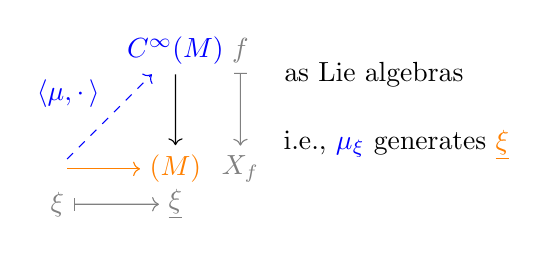
\begin{tikzpicture}[scale=1.5]
			\node[orange] (A) at (0,0) {$\g$};
			\node[gray] (A1) at (0,-.3) {$\xi$};
			\node[blue] (B) at (1,1) {$C^\infty(M)$};
			\node[gray] (B2) at (1.55,1) {$f$};
			\node[orange] (C) at (1,0) {$\X(M)$};
			\node[gray] (C1) at (1,-.3) {$\underline\xi$};
			\node[gray] (C2) at (1.55,0) {$X_f$};
	
			\path[->,blue,dashed] (A) edge node[above left] {$\langle\mu,\cdot\,\rangle$} (B);
			\path[->,orange] (A) edge (C);
			\path[->] (B) edge (C);
			\path[|->,gray] (A1) edge (C1);
			\path[|->,gray] (B2) edge (C2);
	
			\begin{scope}[xshift=3cm]
				\node at (-.32,.8) {as Lie algebras};
				\node at (-.13,.2) {i.e., {\color{blue}$\mu_\xi$} generates {\color{orange}$\underline\xi$}};
			\end{scope}
		\end{tikzpicture}
		
			\footnotesize		(\emph{moment map:} ${\color{blue}\mu:M\to\g^*}$, 
		 \emph{Hamiltonian $G$-space:} 	$(M,\omega,G,\mu)$)
		\end{center}
		\item
		 $\alpha\mapsto X_\alpha$ is a homomorphism of Leibniz algebras:
		$$\d\{\alpha,\beta\} = \d\L_{X_\alpha}\beta = \L_{X_\alpha}\iota_{X_\beta}\omega = \iota_{[X_\alpha,X_\beta]}\omega ~{\color{black!80} \implies}~
		X_{\{\alpha,\beta\}} = [X_\alpha,X_\beta]$$
}
%- . - . - . - . - . - . - . - . - . - . - . - . - . - . - . - . - . - . - . - . - . - . - . - .%


%- . - . - . - . - . - . - . - . - . - . - . - . - . - . - . - . - . - . - . - . - . - . - . - .%
\begin{frame}[fragile]{Marsden-Weinstein-Meyer reduction}
	\begin{thmblock}[Marsden-Weinstein reduction \cite{MarsdenWeinstein74}]
		\vspace{-.4em}\hspace{-1em}
		\begin{tabular}{l p{14cm}}
			Given: & $(M,\omega)$ symplectic
			\\
			& $\color{orange}G\curvearrowright M$ symplectic with equivariant momap. $\mu:M\to \mathfrak{g}^*$
			\\[.2em]
			Assume: & ${\color{blue}\phi} \in \mathfrak{g}^*$ regular value of $\mu$ 
			\qquad\quad \footnotesize \textcolor{gray}{($\Rightarrow$ $\mu^{-1}(\phi)\hookrightarrow M$ smooth embedding)}
			\\
			& $G_\phi\curvearrowright \mu^{-1}(\phi)$ free and proper
			\quad \footnotesize \textcolor{gray}{($\Rightarrow$ $\mu^{-1}(\phi)/G_\phi$ smooth manifold)}
			\\[.4em]
			Then: & \textbf{$\exists!$ symplectic structure} $\omega_\phi$ in $M_\phi:={\color{blue}\mu^{-1}(\phi)}{\color{orange}/G_\phi}$ \\
			& s.t. $\pi^\ast \omega_\phi = j^\ast \omega$ 
			\qquad {\footnotesize with $j:\mu^{-1}(\phi) \hookrightarrow M$ and $\pi:\mu^{-1}(\phi)\twoheadrightarrow M_\mu$}
		\end{tabular}
		\vspace{-.4em}
	\end{thmblock}
	%
	\vfill
	\begin{center}
	\begin{tikzpicture}[scale=2]
		\node[blue] (A) at (0,0) {$\mu^{-1}(\phi)$};
		\node[gray] (A1) at (0,.3) {$i^*\omega$};
		\node[gray] (A2) at (-.6,0) {$\pi^*\omega_\phi$};
		\node[blue] (B) at (1,0) {$M$};
		\node[gray] (B1) at (1,.3) {$\omega$};
		\node[orange] (C) at (0,-.8) {$M_\phi$};
		\node[gray] (C2) at (-.6,-.8) {$\omega_\phi$};

		\path[right hook->,blue] (A) edge node[above] {$i$} (B);
		\path[orange,->] (A) edge node[left] {$\pi$} (C);
		\begin{scope}[xshift=-1.8cm]
			\node[blue] at (0,0) {\small restrict to $\{\mu=\phi\}$};
			\node[orange] at (.15,-.4) {\small quotient by $G_\phi$};
		\end{scope}
	\end{tikzpicture}
	\end{center}
	\pause
	\vfill
	\centering
	The action of $G$ on $\mu^{-1}(0)$ is free and proper $\Rightarrow$ $0$ is reg. val. of $\mu$

\end{frame}
\note[itemize]{
 \item 
	Let $(M,\omega)$ symplectic, $G\circlearrowright M$ be a Lie group action\pause and $\mu:M\to \mathfrak g^*$ such that: 
	\item  $\mu$ is a momentum, i.e. the infinitesimal action $\xi\mapsto \underline\xi:\mathfrak g\to \mathfrak X(M)$ of $G$ satisfies $X_{\langle\mu,\xi\rangle}=\underline \xi$. 
	\item $\mu$ is $G$-equivariant, i.e. $\mu(gm)=Ad^*_g\mu(m)$ 
	\item Then $\exists!$ symplectic form $\omega_r$ on $M_r=\frac{\mu^{-1}(0)}{G}$ such that $\pi^*\omega_r=i^*\omega$.
%% https://q.uiver.app/#q=WzAsMyxbMCwwLCJNIl0sWzMsMCwiXFxtdV57LTF9KDApIl0sWzYsMCwiTV9yIl0sWzEsMCwiaVxcXFwgXFxzdWJzdGFja3tpbmNsdXNpb25+b2Z+c3Vic3BhY2V9IiwyLHsic3R5bGUiOnsidGFpbCI6eyJuYW1lIjoiaG9vayIsInNpZGUiOiJib3R0b20ifX19XSxbMSwyLCJcXHBpXFxcXCBcXHN1YnN0YWNre3F1b3RpZW50fmJ5fnJlbGF0aW9ufSJdXQ==
%\[\begin{tikzcd}
%	M &&& {\mu^{-1}(0)} &&& {M_r}
%	\arrow["\begin{array}{c} i\\ \substack{inclusion~of~subspace} \end{array}"', hook', from=1-4, to=1-1]
%	\arrow["\begin{array}{c} \pi\\ \substack{quotient~by~relation} \end{array}", two heads, from=1-4, to=1-7]
%\end{tikzcd}\]

}
%- . - . - . - . - . - . - . - . - . - . - . - . - . - . - . - . - . - . - . - . - . - . - . - .%


 


%- . - . - . - . - . - . - . - . - . - . - . - . - . - . - . - . - . - . - . - . - . - . - . - .%
\subsection{Singular reduction}
\begin{frame}{Symplectic singular reduction schemes}
	\begin{block}{The gist of singular reduction}
		 \begin{itemize}
			 \item[-] when $\mu$ is singular (i.e. $\mu^{-1}(0)$ is not a mfd.), the (geometrically) reduced space may not exist.
			 \item[-] a \emph{singular reduction scheme} is a procedure to construct a "reduced" algebra of observable out of the given data
			 \item[-] such that it corresponds to the algebra of observable of the reduced manifold in the regular case.
		 \end{itemize}
	\end{block}
	 %
	 \pause
	 \vfill
	 %
	\begin{thmblock}[Sniatycki-Weinstein reduction \cite{SniatyckiWeinstein83}]
		\vspace{-.4em}\hspace{-1em}
		\begin{tabular}{l p{14cm}}
			Given: & $(M,\omega)$ symplectic
			\\
			& $G\curvearrowright M$ symplectic with equivariant momap. $\mu:M\to \mathfrak{g}^*$
			\\[.4em]
			Then: & 
			$\displaystyle \left[\sfrac{C^\infty(M)}{I_\mu}\right]^G$
			admits a Poisson algebra structure 
			\footnote{$I_\mu$ = associative ideal generated by $\widetilde{\mu}(\g)$}			
			\\
			& it agrees with the M--W reduction in the regular case.		
		\end{tabular}
		\vspace{-.4em}
	\end{thmblock}
 \end{frame}
\note[itemize]{
 \item Let $(M,\omega,G,\mu)$ be a symplectic Hamiltonian $G$-space.
 \item The \emph{momentum ideal} is the associative ideal $I_\mu\subset C^\infty(M)$ generated by the momenta $\mu_{\xi}$ for any $\xi\in \mathfrak{g}$.
		Namely
		\[
			I_\mu 
			= 
			\Big\langle \mu_\xi \Big\rangle_{\xi \in \mathfrak{g}}^{\text{\tiny asso.}} 
			=
			\left\{
				\left.
					\sum_{i=1}^n f_i ~ \mu_{\xi_i}
				\right|~
					f_i \in C^\infty(M),~ \xi_i\in \mathfrak{g},~  1 \leq i \leq n
			\right\}
		\]

 \item The \emph{\'Sniatycki--Weinstein reduction} is the Poisson algebra
		\[
			\left(C^\infty(M)/I_\mu\right)^G.
		\]


}
%- . - . - . - . - . - . - . - . - . - . - . - . - . - . - . - . - . - . - . - . - . - . - . - .%	











%- . - . - . - . - . - . - . - . - . - . - . - . - . - . - . - . - . - . - . - . - . - . - . - .%
\subsection{Constraints Algebras}
\begin{frame}[fragile]{Attempting algebraic reduction naively}
When the action is not 'free and proper', we can try to mimic this directly using the function algebras:
% https://q.uiver.app/#q=WzAsNixbMCwwLCJNIl0sWzEsMCwiXFxtdV57LTF9KDApPVMiXSxbMywwLCJNX3IiXSxbMCwxLCJDXlxcaW5mdHkoTSkiXSxbMSwxLCJDXntcXGluZnR5fShTKT1cXGZyYWN7Q157XFxpbmZ0eX0oTSl9e0lfe1N9fSJdLFszLDEsIkNee1xcaW5mdHl9KE1fcik9Q15cXGluZnR5KFMpXkciXSxbMSwyLCJcXHN1YnN0YWNre3F1b3RpZW50fSIsMCx7InN0eWxlIjp7ImhlYWQiOnsibmFtZSI6ImVwaSJ9fX1dLFszLDQsIlxcc3Vic3RhY2t7cXVvdGllbnR9IiwwLHsic3R5bGUiOnsiaGVhZCI6eyJuYW1lIjoiZXBpIn19fV0sWzAsMSwiXFxzdWJzdGFja3tyZXN0cmljdGlvbn0iLDAseyJzdHlsZSI6eyJib2R5Ijp7Im5hbWUiOiJzcXVpZ2dseSJ9fX1dLFs0LDUsIlxcc3Vic3RhY2t7cmVzdHJpY3Rpb259IiwwLHsic3R5bGUiOnsiYm9keSI6eyJuYW1lIjoic3F1aWdnbHkifX19XV0=
\[\begin{tikzcd}
	M & {\mu^{-1}(0)=S} && {M_r} \\
	{C^\infty(M)} & {C^{\infty}(S):=\frac{C^{\infty}(M)}{I_{S}}} && {C^{\infty}(M_r)=C^\infty(S)^G}
	\arrow["{\substack{restriction}}", squiggly, from=1-1, to=1-2]
	\arrow["{\substack{quotient}}", two heads, from=1-2, to=1-4]
	\arrow["{\substack{quotient}}", two heads, from=2-1, to=2-2]
	\arrow["{\substack{restriction}}", squiggly, from=2-2, to=2-4]
\end{tikzcd}\]

where $I_S=\{f\in C^{\infty}(M)~|~f|_S=0\}$.
\pause 
\vfill
Equivalently:

% https://q.uiver.app/#q=WzAsMyxbMCwwLCJDXlxcaW5mdHkoTSkiXSxbMiwwLCJOX1M9XFx7Zn58fiBmXFxpbiBDXlxcaW5mdHkoTSl8X1N+fkdcXG1hdGhybXstaW52YXJpYW50fVxcfSJdLFs0LDAsIlxcZnJhY3tOX1N9e0lfU30iXSxbMCwxLCJcXHN1YnN0YWNre3Jlc3RyaWN0aW9ufSIsMCx7InN0eWxlIjp7ImJvZHkiOnsibmFtZSI6InNxdWlnZ2x5In19fV0sWzEsMiwiXFxzdWJzdGFja3txdW90aWVudH0iLDAseyJzdHlsZSI6eyJoZWFkIjp7Im5hbWUiOiJlcGkifX19XV0=
\[\small\begin{tikzcd}
	{C^\infty(M)} && {N_S=\{f~|~ f\in C^\infty(M)|_S~~G\mathrm{-invariant}\}} && {\frac{N_S}{I_S}}
	\arrow["{\substack{restriction}}", squiggly, from=1-1, to=1-3]
	\arrow["{\substack{quotient}}", two heads, from=1-3, to=1-5]
\end{tikzcd}\]
\pause
\vfill

\begin{alertblock}{Problem}
	$C^\infty(S)^G=\frac{N_S}{I_S}$ is not a Poisson algebra in general.
\end{alertblock}
(when constraints not first class, cf. Dirac reduction)
\end{frame}
\note[itemize]{
	\item \emph{(Credits to \href{https://www.ryvkin.eu/}{Leonid Ryvkin} for the tex code of this slide.)}
}
%- . - . - . - . - . - . - . - . - . - . - . - . - . - . - . - . - . - . - . - . - . - . - . - .%

%- . - . - . - . - . - . - . - . - . - . - . - . - . - . - . - . - . - . - . - . - . - . - . - .%
\begin{frame}{Constraint Algebras} 
	\begin{block}{Idea:}
	    \begin{itemize}[noitemsep,topsep=0pt,parsep=0pt,partopsep=0pt]
			\item[-] Both regular/geometric and singular/algebraic reduction are 2-steps procedures (1. restrict 2. quotient).
			\item[-] Let's work in a category where all data needed for the reduction are bundled together in a suitable categorical objects. {\tiny (To avoid pathologies arising from these steps)}
	    \end{itemize}
	\end{block}
	\pause
	\vfill
	\begin{defblock}[Constraint algebra triples \cite{Dippell2023}]
		A (strong embedded) constraint algebra $\mathcal A$ is given by a triple $(\mathcal A_T, \mathcal A_N, \mathcal A_0)$, where
		\begin{itemize}[noitemsep,topsep=0pt,parsep=0pt,partopsep=0pt]
			\item[•] $\mathcal A_T$ is an algebra \emph{("total space")}
			\item[•] $\mathcal A_N\subset \mathcal A_T$ a subalgebra  \emph{("normal space")}
			\item[•] $\mathcal A_0\subset \mathcal A_N$ a two-sided ideal in $\mathcal A_T$ \emph{("zero space")}
		\end{itemize}
	\end{defblock}
	\vfill
	\pause
	\begin{exblock}
		Let $S$ be a closed set. Algebraically, we describe $C^\infty(S)$ by $\frac{C^\infty(M)}{I_S}$.
		\\ 
		We can think of it as the constraint triple:
		$$
			\mathcal A=(\mathcal A_T,\mathcal A_N,\mathcal A_0)=(C^\infty(M),C^\infty(M), I_S)
		$$
	\end{exblock}

\end{frame}
\note[itemize]{
	\item  triples of the type (algebra , subalgebra, ideal).
	\item After \cite{Dippell2023} we call such triples { \bf constraint triples} and their parts \emph{total space, normal space, zero space}.
	\item It is a (strong) constraint algebra if $\mathcal A_0\subset \mathcal A_N\subset \mathcal A_T$ subalgebras and $\mathcal A_0\subset \mathcal A_T$ ideal.
}
%- . - . - . - . - . - . - . - . - . - . - . - . - . - . - . - . - . - . - . - . - . - . - . - .%



%- . - . - . - . - . - . - . - . - . - . - . - . - . - . - . - . - . - . - . - . - . - . - . - .%
\begin{frame}{Other approaches to singular reduction}
 	Many singular reduction schemes adhere to this pattern!
 	\vfill
 	\pause
\begin{table}[]
	\begin{tabular}{l|l|l||l}
		algebra $\mathcal{A}_T$ & subalgebra $\mathcal{A}_N$ & ideal $\mathcal{A}_0$ & comment \\
		\hline
		
		$C^\infty(M)$&      $N_S$     &   $I_S$   &  $\substack{S=\mu^{-1}(0),~ I_S=\{f~|~f|_S=0\}}$ \\
			&&&  $\substack{N_S= \{ f | gf-f\in I_S \forall g\in G\}}$ \\
	& & & \color{red} not Poisson \\ 
	\hline	\pause
	$C^\infty(M)$&   $F_S$         &   $I_S$   &  $\substack{F_S=\{f~|~\{f,I_S\}\subset I_S\}}$ \\
	& & & \color{red} if $I_S\subset F_S$\\
	\hline \pause
	
	$C^\infty(M)$&   $C^\infty(M)^G$         &   $(I_S)^G$   &  $\substack{C^\infty(M)^G=\{f~|~gf=f\forall g\in G\}}$ \\
	\hline \pause
		$C^\infty(M)$&   $C^\infty(M)^G$         &   $(I_\mu)^G$   & $\substack{I_\mu=\{\sum_{i=1}^k f_i\langle \mu,\xi_i\rangle|~f_i\in C^\infty(M), \xi_i\in \mathfrak g\}}$\\
		\hline \pause
	$C^\infty(M)$&      $N_\mu$     &   $I_\mu$   & $\substack{N_\mu= \{ f | gf-f\in I_\mu \forall g\in G\}}$ \footnote{When $G$ connected $N_\mu=N(I_\mu):=\{f~|~\{f,I_\mu\}\subset I_\mu\}$.}\\
	\hline 
		
	\end{tabular}\pause
\end{table}
	\vfill
	{\bf Remarks }names in order: 'naive' , Dirac, Sniatycki, Arms-Cushman-Gotay, Sniatycki-Weinstein.

\end{frame}
\note[itemize]{
	\item \emph{(Credits to \href{https://www.ryvkin.eu/}{Leonid Ryvkin} for the tex code of this slide.)}
}
%- . - . - . - . - . - . - . - . - . - . - . - . - . - . - . - . - . - . - . - . - . - . - . - .%
 




%------------------------------------------------------------------------------------------------
\section{Multisymplectic Geometry}
\checkpoint	
%------------------------------------------------------------------------------------------------
 
%- . - . - . - . - . - . - . - . - . - . - . - . - . - . - . - . - . - . - . - . - . - . - . - .%
\subsection{Multisymplectic manifolds}
\begin{frame}{From symplectic to {multi}symplectic} 
	%
	\begin{center}
		$-$ \emph{multisymplectic means \textbf{going higher} in the degree of $\omega$} $-$
	\end{center}
	\pause
	\begin{defblock}[$n$-plectic manifold ~\emph{(Cantrijn, Ibort, De Le\'on)} \cite{Cantrun2017}]
		\includestandalone[width=0.95\textwidth]{Pictures/Figure_multisym}	
	\end{defblock}
	%
	\pause
		\begin{table}
			\begin{tabular}{c c c}
				symplectic forms \small($n=1$) & $\leftrightsquigarrow$ & volume forms \small($n= \text{dim}(M)-1$)
			\end{tabular}
		\end{table}

	\vfill
	\pause
	\begin{block}{Historical motivation}
		Mechanics: geometrical foundations of \textit{(first-order)} field theories.
	\end{block}
	%
	\begin{table}
		\ifHandout
		%
		\else
		\only<4>{
		\begin{tabular}{|p{0.2\textwidth}|p{0.3\textwidth}|p{0.35\textwidth}|} 
            \hline
            \parbox[][20pt][c]{0.2\textwidth}{mechanics} & \multicolumn{2}{c|}{geometry} \\
            \hline
            \parbox[][20pt][c]{0.2\textwidth}{phase space} & symplectic manifold &  \\[.25em]
            \parbox[][20pt][c]{0.2\textwidth}{classical \\ observables} & Poisson algebra &  \\[.25em]
            \parbox[][20pt][c]{0.2\textwidth}{symmetries} &  group actions admitting comoment map &  
            \\
            \hline
  \multicolumn{1}{c}{}
            &  \multicolumn{1}{@{}c@{}}{$\underbrace{\hspace*{.3\textwidth}}_{\text{point-like particles systems}}$} 
            &  \multicolumn{1}{@{}c@{}}{}              \\
		\end{tabular}
		}
		\fi
		\onslide<5->{
		\begin{tabular}{|p{0.2\textwidth}|p{0.3\textwidth}|p{0.35\textwidth}|} 
            \hline
            \parbox[][20pt][c]{0.2\textwidth}{mechanics} & \multicolumn{2}{c|}{geometry} \\
            \hline
            \parbox[][20pt][c]{0.2\textwidth}{phase space} & symplectic manifold & multisymplectic manifold \\[.25em]
            \parbox[][20pt][c]{0.2\textwidth}{classical \\ observables} & Poisson algebra & $L_\infty$-algebra \\[.25em]
            \parbox[][20pt][c]{0.2\textwidth}{symmetries} &  group actions admitting comoment map & group actions admitting (homotopy) comomentum map
            \\
            \hline
  			\multicolumn{1}{c}{}
            &  \multicolumn{1}{@{}c@{}}{$\underbrace{\hspace*{.3\textwidth}}_{\text{point-like particles systems}}$} 
            &
            \multicolumn{1}{@{}c@{}}{$\underbrace{\hspace*{.3\textwidth}}_{\text{field-theoretic systems}}$} 
               \\
		\end{tabular}
		}
	\end{table}	




\end{frame}
\note[itemize]{
	\item Historically, the interest in multisymplectic manifolds, has been motivated by the need for understanding the geometrical foundations of first-order classical field theories.
	The key point is that, just as one can associate a symplectic manifold to an ordinary classical mechanical system (e.g. a single
point-like particle constrained to some manifold), it is possible to associate a multisymplectic
manifold to any classical field system (e.g. a continuous medium like a filament or a fluid). See frame Extra-\ref{Frame:Ms-Field-Mechanics} 
	
	\item General ideas basic parallelisms with caveats
	\item caveat: points in multiphase spaces are not states
	\item the table hides the duality between geometric and algebraic approaches to the problem.
	\item	Mechanics: geometrical foundations of \textit{(first-order)} field theories.
		\begin{itemize}
		 \item[-] Kijowski, W. Tulczyjew \cite{Kijowski1979}; %(1979)
		 \item[-] Cariñena, Crampin, Ibort \cite{Carinena1991b};% (1991)
		 \item[-] Gotay, Isenberg, Marsden, Montgomery \cite{Gimmsy1};%(1998)
		 \\ $\cdots$
		\end{itemize}
	\item {Def. Multisymplectic manifold $(M,\omega)$}
	$M$ a smooth manifold, $\omega\in \Omega^{n+1}(M)$ closed and non-deg., i.e.: $d\omega=0$ and $\omega^\flat:TM\to \Lambda^nT^*M, v\mapsto \iota_v\omega$ is injective.
	\item Examples: orientable $n{+}1$-manifolds with volume (e.g. $S^{n+1}$, $T^{n+1}$, $\mathbb R^{n+1}$ ), multicotangent bunlde $\Lambda^nT^*Q$ of any manifold $Q$ (with $\omega=d\theta$. $\theta_\eta(v_1,...,v_n)=\eta(T\pi_Q(v_n),...,T\pi_Q(v_n))$),  semisimple Lie groups, hyperKähler manifolds,...
 	\item Without the non-deg. condition we call it \emph{premultisymplectic}. 

}
%- . - . - . - . - . - . - . - . - . - . - . - . - . - . - . - . - . - . - . - . - . - . - . - .%


%- . - . - . - . - . - . - . - . - . - . - . - . - . - . - . - . - . - . - . - . - . - . - . - .%
\subsection{Higher Observables}
\begin{frame}{Observables in $n$-plectic geometry}
	%
	\begin{defblock}[Hamiltonian $(n-1)$-forms]
		\begin{displaymath}
			\Omega^{n-1}_{ham}(M,\omega) 	:=
			\biggr\{ \sigma \in  \Omega^{n-1}(M) \; \biggr\vert \; 
				\exists \vHam_\sigma \in \mathfrak{X}(M) ~:~ 
				\tikz[baseline,remember picture]{\node[rounded corners,
                        fill=orange!5,draw=orange!30,anchor=base]            
            			(target) {$d \sigma = -\iota_{\vHam_\sigma} \omega$ };
            	}				
				~\biggr\} 
		\end{displaymath}
	\end{defblock}
%
%	\pause
%		\tikz[overlay,remember picture]
%		{
%			\node[rounded corners,
%                 fill=orange!5,draw=orange!30,anchor=base]
%            	 (base) at ($(current page.north east)-(2,1)$) [rotate=-0,text width=3.5cm,align=center] {\footnotesize{\textcolor{red}{Hamilton-DeDonder-Weyl \\equation}}};
%		}	
%	\begin{tikzpicture}[overlay,remember picture]
%    	\path[->] (base.south) edge[bend right,red](target.north);
%    \end{tikzpicture}
	%
	\vfill
	\begin{columns}[T]
		\pause
		\setlength{\belowdisplayskip}{5pt}
		\begin{column}{.50\linewidth}
			%
			\vspace{-1em}
			\begin{thmblock}[Observables $L_\infty$-algebra]
				$\Omega^{n-1}_{ham}(M,\omega)$ endowed with
				\vspace{-.5em}
				\begin{displaymath}
					\lbrace \sigma_1, \sigma_2 \rbrace =			
					~ - \iota_{\vHam_1}\iota_{\vHam_2} \omega 
				\end{displaymath}			
				can be "completed" to a \\ $L_\infty-algebra$.
			\end{thmblock}
			%	
		\end{column}	
		%
		\pause
		\begin{column}{.50\linewidth}
		%
			\begin{itemize}
				\item[\cmark] Skew-symmetric;
				\item[\xmark] multiplication of observables;
				\item[\xmark] Jacobi equation;
				%\\ \hspace*{4.25em} full-fledged Jacobi equation;
				\item[\smark] Jacobi equation \emph{up to homotopies}.
			\end{itemize}			
			%
				\[
					\small
					\{\alpha,\{\beta,\gamma\}\} + \text{\it cyc. perm.}
					= {\color{orange}\d \iota_{X_\alpha} \iota_{X_\beta} \iota_{X_\gamma}\omega}
				\]
		\end{column}	
	\end{columns}
	%
	\vfill
	\pause
	Interesting alternatives:
	\begin{itemize}
		\item  descend to $\Omega^{n-1}_{ham}(M) / {\color{orange}\d\hspace{1pt}\Omega^{n-2}(M)}$, hence getting a Lie algebra;
		\item Incorporate the {\color{orange}discrepancy} as part of the data of the space of observables $ 
				L_\infty(M,\omega) = \Omega_{ham}^{n-1}(M)\oplus{\color{orange}\Omega^{\leq n-2}(M)}$.
			%a \textbf{homotopy Lie algebra} or \textbf{$L_\infty$-algebra}.
	\end{itemize}
	
	
\end{frame}
\note[itemize]{
	\item In the paper 
 \href{https://www.sciencedirect.com/science/article/pii/S0393044018301189}{Invitation to Multisymplectic Geometry} \cite{RYVKIN20199}\	, the equation highlighted in orange, which defines Hamiltonian forms, is referred to as the Hamilton--DeDonder--Weyl equation---a somewhat imaginative extension compared to its traditional formulation in \href{https://en.wikipedia.org/wiki/De_Donder\%E2\%80\%93Weyl_theory}{De Donder--Weyl theory}. 
}
%- . - . - . - . - . - . - . - . - . - . - . - . - . - . - . - . - . - . - . - . - . - . - . - .%



%- . - . - . - . - . - . - . - . - . - . - . - . - . - . - . - . - . - . - . - . - . - . - . - .%
\begin{frame}[fragile,t]{$L_\infty$-algebra of Observables (higher observables) }
	Let be $(M,\omega)$ a $n$-plectic manifold.
	\begin{defblock}[$L_\infty$-algebra of observables ~\emph{(Rogers)} ~\cite{Rogers2010}]
		
		\hspace{.25em} $L\infty(M,\omega)$ is given by:
		
		\begin{itemize}
			\item[•] a cochain-complex $(L,\{\cdot\}_1)$ 
		\end{itemize}
		\begin{center}
		\ifHandout
			\includestandalone{Pictures/Figure_Observables}	
		\else
			\includestandalone{Pictures/Frame_Observables}
		\fi				
		\end{center}
		\onslide<2->{
			\begin{itemize}
				\item[•] with $n$ (skew-symmetric) multibrackets $(2 \leq k \leq n+1)$
			\end{itemize}
			\begin{center}
				\includestandalone{Pictures/Equation_Multibracket}	
			\end{center}
		}
		%
	\end{defblock}
  \end{frame}
 \note[itemize]{
	\item if symplectic manifolds are the symmetric take on mechanics, Poisson algebras are the algebraic counterpart.
 	\item A Lie algebra is associated to an ordinary symplectic manifold (its Poisson algebra).
	%(Underlying this is a Lie algebra, whose Lie bracket is the Poisson bracket.)
	Similarly, one associates an Lie-$n$ algebra to any $n$-plectic manifold.
 	% https://ncatlab.org/nlab/show/n-plectic+geometry 	 
 	 %https://ncatlab.org/nlab/show/Poisson+bracket+Lie+n-algebra
	 \item Basically, the higher observables algebra is a chunk of the de Rham complex of $M$ with inverted grading( convention employed here) and an extra structure called "multibrackets".
 	\item ( In the 1-plectic case it reduces to the corresponding Poisson algebra of classical observables)
 	\item Rogers associated to any n-plectic mfd a $L\-\infty$ algebra, Zambon generalized it to the pre-n-plectic case.
 	\item Recognize in the definition of $\{\cdot,\ldots,\cdot\}_k$ the contraction with hamiltonian fields $v_\sigma$ w.r.t. $\sigma$.
  	\item Note $	\iota_{v_{\sigma_1}}\cdots\iota_{v_{\sigma_k}} = (-)^{(k-1)+(k-2)+\dots+1}\iota_{v_{\sigma_k}}\cdots\iota_{v_{\sigma_1}} = (-)^{\frac{k(k-1)}{2}}\iota_{v_{\sigma_k}}\cdots\iota_{v_{\sigma_1}}$ 
 	The definition usually find in literature of Rogers multibrackets involves the coefficient $ (-)^{\frac{k(k-1)}{2}} = -\varsigma(k-1) = (-)^{k+1} \varsigma(k)$.
  \item higher observables is Special instance of a more general object  called $L\-\infty$ Algebra...
 }
%- . - . - . - . - . - . - . - . - . - . - . - . - . - . - . - . - . - . - . - . - . - . - . - .%


%------------------------------------------------------------------------------------------------
\section{Multisymplectic observables reduction}
\checkpoint	
%------------------------------------------------------------------------------------------------
 
 %- . - . - . - . - . - . - . - . - . - . - . - . - . - . - . - . - . - . - . - . - . - . - . - .%
\subsection{General idea}
\begin{frame}{Singular Reduction: Roadmap}
	%
	\begin{block}{Data:}
			\begin{itemize}
				\item $(M,\omega)$ multisymplectic,
				\item $S\subset M$ closed subset (possibly singular),
				\item $I_S$ the ideal of smooth functions vanishing on $S$,
				\item $F\subset \mathfrak X(M)$ a Lie subalgebra s.th. $F(I_S)\subset I_S$.
			\end{itemize}
	\end{block}
	%
	\vfill
	\pause
	%
	\begin{block}{Goal:}
		\begin{itemize}
			\item Identify a constraint triple of the type (algebra , subalgebra, ideal) pertaining to the $L_\infty$ algebra of observables.
		\end{itemize}
	\end{block}
	%
	\vfill
	\pause
	%
	\begin{block}{Strategy:}
		\begin{enumerate}
			\item Define smooth fields/forms \emph{tangent to $N$},
			\item define smooth fields/forms \emph{vanishing along $N$},
			\item define \emph{reducible fields} requiring the preservation of the vanishing objects,
			\item define \emph{reducible forms} requiring their conservation w.r.t. the infinitesimal action,
			\item define \emph{reducible and vanishing observables},
			\item \textbf{quotient}
		\end{enumerate}
	\end{block}






\end{frame}
\note[itemize]{
	\item Remark: the following singular reduction scheme is slightly different from what we proposed in our paper \cite{Blacker2022}.
}
 %- . - . - . - . - . - . - . - . - . - . - . - . - . - . - . - . - . - . - . - . - . - . - . - .% 
 
 %- . - . - . - . - . - . - . - . - . - . - . - . - . - . - . - . - . - . - . - . - . - . - . - .%
\begin{frame}{Translating geometry to algebra}

	\vfill
	\begin{table}[]
		\begin{tabular}{l|l|l}
		 geometry & algebra & translation \\
			\hline	
		smooth manifold $M$ & comm. algebra $\mathcal A_T$  	& $\mathcal A_T=C^{\infty}(M)$\\ \hline\pause
		vector fields $\mathfrak X(M)$ & derivations $\Der(\mathcal A_T)$ &  $\Der(C^\infty(M))=\mathfrak X(M)$\\ \hline\pause
		closed subset $S\subset M$ & ideals $\mathcal A_0\subset \mathcal A_T$ & $\mathcal A_0=I_S=\{f~|~f|_S=0\}$ \\ \hline\pause
		action $G\circlearrowleft M$ & Lie algebra map & infinitesimal generators\\
		 of connected group &$\underline{\cdot}:\mathfrak g\to \Der(\mathcal A_T)$ & of the action \\ \hline \pause
		 $G$ action preserves $S$ & $\underline \xi(I_S)\subset I_S$ $\forall \xi\in\mathfrak g$& \color{red} Careful! Not equivalent! 
		 \\ \hline
		\end{tabular}
	\end{table}
	\vfill


\end{frame}
\note[itemize]{
	\item \emph{(Credits to \href{https://www.ryvkin.eu/}{Leonid Ryvkin} for the tex code of this slide.)}
	\item {Warning}
	$\partial_x$ is algebraically preserving $S=[0,1]\subset \mathbb R=M$, even though the flow leads out of the set.
}
%- . - . - . - . - . - . - . - . - . - . - . - . - . - . - . - . - . - . - . - . - . - . - . - .%







%- . - . - . - . - . - . - . - . - . - . - . - . - . - . - . - . - . - . - . - . - . - . - . - .%
\subsection{Higher Observables Constraint Algebra}
\begin{frame}[shrink]{Higher Observables Constraint Algebra}
	\begin{defpropblock}[$L_\infty$-observables constraint algebra]
		The following $L_\infty$ algebra\footnote{ 
			\vspace{-1.75em}
			\begin{align*}
				\small \text{where:\quad} &\Omega_0^k ~:=&\{\alpha \in \Omega^k(M)~|~\alpha(v_1,...,v_k)\in  I_S~\forall v_i\in \X_N\} 
				\\
				& \mathfrak{X}_N ~:=& 
				\left\lbrace
					v \in \X(M)
				~\left\vert~
					\begin{array}{l}
						\L_v (I_N) \subseteq I_N	\\		
						\L_v (C^{\infty}(M) F) \subseteq C^{\infty}(M) F + I_S\mathfrak X(M)
					\end{array}
				\right\rbrace\right.
			\end{align*} 
		} form a constraint triple
		\begin{align*}
			\Ham_T =&~ L_\infty(M,\omega) \\[1em]
			\Ham_N =&~
			{\small
			\left\lbrace
			\begin{array}{l}
				\alpha\in \Omega^{\leq n-2}(M) \\\mathrm{\small, respectively}\\	
				(\alpha,X) \in \Omega^{n{-}1}(M) \oplus\mathfrak X(M)
			\end{array}
			~\left\vert~
			\begin{array}{l l}
				\iota_\xi \alpha \in \Omega_0 &\\
				\L_\xi\alpha \in \Omega_0&~\forall \xi \in F\\
				\hline
				\iota_X \omega = -d \alpha &\\
				X(I_S)\subset I_S &\\
				\L_\xi X \in C^{\infty}(M) F + I_S\mathfrak X(M)
				&~\forall \xi \in F\\
			\end{array}
			\right.
			\right\rbrace 
			}
			\\[1em]
			\Ham_0 =&~
		{\small
			\left\lbrace
			\begin{array}{l}
				\alpha\in \Omega^{\leq n-2}(M) \\\mathrm{\small, respectively}\\	
				(\alpha,X) \in \Omega^{n{-}1}(M) \oplus\mathfrak X(M)
			\end{array}
			~\left\vert~
			\begin{array}{l}
				\alpha \in \Omega_0\\
				\hline
				\iota_X \omega = -d \alpha\\
				X \in C^{\infty}(M) F + I_S\mathfrak X(M)
			\end{array}
			\right.
			\right\rbrace
		}
		\end{align*}
	\end{defpropblock}
	\vfill
	\pause
	{\centering \color{red} $\Rightarrow$  the subquotient ${\Ham_N} / {\Ham_0}$ forms an $L_\infty$-algebra!}
\end{frame}
\note[itemize]{
	\item 	
	\begin{defblock}[Reducible v.fields ]
			\begin{displaymath}
				\mathfrak{X}_N ~:=
				\left\lbrace
					v \in \X(M)
				~\left\vert~
					\begin{array}{l}
						\L_v (I_N) \subseteq I_N	\\		
						\L_v (C^{\infty}(M) F) \subseteq C^{\infty}(M) F + I_S\mathfrak X(M)
					\end{array}
				\right\rbrace\right.
			\end{displaymath}
			e.g. $F=\X_g$ is the $C^\infty(M)$-module generated by the fundamental distribution of an acting group.
	\end{defblock}	
	%
	\begin{defblock}[Reducible forms ]
		\begin{displaymath}
			\Omega_{N} :=
			\left\lbrace
				\alpha \in \Omega(M)
			~\left\vert~
				\begin{array}{l r}
					\L_\underline{\xi} \,\alpha \in \Omega_0	\\		
					\iota_\underline{\xi} \,\alpha \in \Omega_0	& \forall \xi \in \g				\end{array}
			\right\rbrace\right.
		\end{displaymath}	
	\end{defblock}	
	%
	%
	\begin{defblock}[Reducible Hamiltonian forms]
		\begin{displaymath}
			(\Omega(M)_{ham}^{n-1})_{[N]} :=
			\left\lbrace
				\alpha \in \Omega(M)_{ham}^{n-1}
			~\left\vert~
				\begin{array}{l r}
					\alpha \text{ is a reducible form} \\
					\vHam_\alpha \text{ is a reducible v.field}
				\end{array}
			\right\rbrace\right.
		\end{displaymath}	
	\end{defblock}	
}
%- . - . - . - . - . - . - . - . - . - . - . - . - . - . - . - . - . - . - . - . - . - . - . - .%

%- . - . - . - . - . - . - . - . - . - . - . - . - . - . - . - . - . - . - . - . - . - . - . - .%
\subsection{Conclusions}
%TODO questa slide non è leggibile!
\begin{frame}{Conclusions}
	\begin{itemize} 
\item Constraint triples permit to do differential geometry/ Cartan calculus on singular subquotients,\\ ... in particular constructing observable algebras on them.\pause
\item Even if $\omega$ is non-degenerate, $\omega_r$ could degenerate, forcing us to pull along the Hamiltonian vector fields explicitly\pause
\item Coomentum maps in the sense of the Leibniz structure seem better for reducing than $L_\infty$-comomenta \pause
%\item The algebraic approach can treat algebroid / singular foliation symmetries and remembers vanishing orders a the singularities. \pause
\item The reduction seems to give something novel even in the symplectic case 
\begin{thmblock}[Multisymplectic reduction in the symplectic case \cite{Blacker2022}]
Let $Q=\{f~|~ f|_S=0\rm{~and~} df|_S=0\}$ Then the $L_\infty$-reduction is:
$$
\frac{N(I_S)\cap N(I_\mu+Q)}{I_\mu+Q}
$$
\end{thmblock}

	\pause
			\vfill
		  \centering 
		  {\Huge\color{red} 
		  \emph{Thank you for your attention!}}
			\vfill
	\end{itemize}
\end{frame}
\note[itemize]{
	\item
}
%- . - . - . - . - . - . - . - . - . - . - . - . - . - . - . - . - . - . - . - . - . - . - . - .%





%------------------------------------------------------------------------------------------------
% APPENDIX
%------------------------------------------------------------------------------------------------
\appendix
%------------------------------------------------------------------------------------------------

\section{Supplementary Material}
%- . - . - . - . - . - . - . - . - . - . - . - . - . - . - . - . - . - . - . - . - . - . - . - .%
\begin{frame}
	\begin{center}
	\Huge\emph{Supplementary Material}
	\end{center}
\end{frame}
\note[itemize]{
	\item
}
\addtocounter{framenumber}{-1}
%- . - . - . - . - . - . - . - . - . - . - . - . - . - . - . - . - . - . - . - . - . - . - . - .%


%- . - . - . - . - . - . - . - . - . - . - . - . - . - . - . - . - . - . - . - . - . - . - . - .%
\begin{frame}[fragile]{MS geometry and classical field mechanics}\label{Frame:Ms-Field-Mechanics}
		Consider a smooth manifold $Y$,
		\begin{columns}
			\hfill
			\begin{column}{.5\linewidth}
				\emph{Multicotangent bundle} $\bigwedge = \bigwedge^n T^\ast Y$\\
				is naturally $n$-plectic
			\end{column}
			\begin{column}{.4\linewidth}
				\[
				\begin{tikzcd}
					\Lambda \ar[d,"\pi"'] & T \Lambda \ar[d,"T \pi"] \ar[l] \\
					Y								& T Y \ar[l]
				\end{tikzcd}	
				\]
			\end{column}
		\end{columns}
	\pause
	\begin{defblock}[Tautological $n$-form]
		$\theta \in \Omega^n(\Lambda)$ such that:
		\begin{displaymath}
		\begin{split}
			\left[ \iota_{u_1 \wedge \ldots \wedge u_n} \theta \right]_\eta 
			&= \iota_{(T \pi)_\ast u_1 \wedge \ldots \wedge (T \pi)_\ast u_n} \eta \\
			&= \iota_{u_1 \wedge \ldots \wedge u_n} \pi^\ast \eta 
			\qquad \qquad \forall \eta \in \Lambda \, , \: \forall u_i \in T_\eta \Lambda 		
		\end{split}
		\end{displaymath}
	\end{defblock}
	\vfill
	\begin{columns}
		\begin{column}{.6\linewidth}
			\begin{defblock}[Tautological (multisymplectic) (n+1)-form]
				$$\omega := d \theta$$
			\end{defblock}
		\end{column}
		\begin{column}{.4\linewidth}
		 	\begin{claimblock}$\omega$ is not degenerate.\end{claimblock}	
		\end{column}
	\end{columns}	
	\pause
	\begin{keywordblock}
		\begin{tabular}{|c|c|c|}
			\hline 
			point-particles mechanics & $\rightsquigarrow$ & classical fields mechanics \\
			%(finite discrete DOF) & & (finite dimensional continuous DOF) \\
			\hline 
			symplectic & $\rightsquigarrow$ & multisymplectic \\ 
			\hline 
			Observables (Poisson) algebra & $\rightsquigarrow$ & Observables $L-\infty$ algebra
			 \\ 
			\hline 
			Co-moment map & $\rightsquigarrow$ & Homotopy co-momentum map \\ 
			\hline 
		\end{tabular} 
	\end{keywordblock}

	
\end{frame}
\note[itemize]{
	\item This example is significant from the perspective of geometric classical field theory:
		\begin{displaymath}
			\frac{\text{classical mechanics}}{\text{symplectic geo.}} =
			\frac{\text{classical field mechanics}}{\text{multisymplectic geo.}}
		\end{displaymath}
	\item Multicotangent bundle is the \emph{Higher analogue} of the cotangent bundle.
	(but it is not yet the analogue of a \emph{phase space}.)
\item The multiphase space is the sub-bundle of $n$-forms vanishing when contracted with 2 vertical fields.
  	\item The reason why this sub-bundle has a particular role is that it can be proved to be isomorphic to a suitable dual of the first Jet bundle.
  	\item For further details see Gotay et al. \href{https://arxiv.org/abs/physics/9801019}{arXiv:physics/9801019}. For a pictorial representation of all the structures involved in the geometric mechanics of I order classical field theories see appendix, pag: \ref{frame:Gimmsy}.
}
%- . - . - . - . - . - . - . - . - . - . - . - . - . - . - . - . - . - . - . - . - . - . - . - .%
	

%- . - . - . - . - . - . - . - . - . - . - . - . - . - . - . - . - . - . - . - . - . - . - . - .%
\begin{frame}[t]{Symmetries in \textbf{multisymplectic geometry}}
	Consider a Lie algebra action $v:\mathfrak{g} \to \mathfrak{X}(M)$  preserving the $n$-plectic form $\omega$,
	\vfill

	\vspace{-1em}
	\begin{columns}[T]
		\setlength{\belowdisplayskip}{5pt}
		\begin{column}{.50\linewidth}
			%
			\centering \it
			\onslide<2->{
				$-$ symplectic case $-$
				\begin{defblock}[Comoment map pertaining to $v$]
					Lie algebra morphism
					$$ f: \mathfrak{g} \to C^\infty(M) $$
					such that
					$$ d~f (x) = -\iota_{v_x} \omega \qquad \forall x \in \mathfrak{g}~.$$
				\end{defblock}
			}
		\end{column}	
		%
		\onslide<2->{\vrule{}}
		%
		\begin{column}{.50\linewidth}
			\centering \it
			\onslide<3->{			
				$-$ $n$-plectic case $-$
				\begin{defblock}[Homotopy comoment map \tiny (HCMM)]
					$L_\infty$-morphism 
					$$ (f_k) : \mathfrak{g} \to L_\infty (M,\omega)$$
					such that
					$$ d~f_1(x) = -\iota_{v_x} \omega \qquad \forall x \in \mathfrak{g}~.$$
				\end{defblock}	
			}
		\end{column}	
	\end{columns}	
	%
	\pause
	\vfill
	\centering 
	\onslide<4->{\textbf{-- Conserved quantities --}}
	%
	\vspace{-.5em}
	\begin{columns}[T]
		\setlength{\belowdisplayskip}{5pt}
		\begin{column}{.50\linewidth}
			%
			\centering \it
			\onslide<4->{
			\begin{propblock}[Noether Theorem]
				\small Fixed $H\in C^\infty_{\text{Ham}}(M)$ ($\mathfrak{g}$-invariant) ,
				$$\mathcal{L}_{v_H} f(x) = 0 \qquad \forall x \in \mathfrak{g}$$
			\end{propblock}
			}
		\end{column}	
		%
		\onslide<5->{\vrule{}}
		%
		\begin{column}{.50\linewidth}
			\centering \it
			\onslide<5->{			
			\begin{propblock}[RWZ16 Theorem]
				\small Fixed $H\in \Omega^{n-1}_{\text{Ham}}(M)$ ($\mathfrak{g}$-invariant),
				$$\mathcal{L}_{v_H} f_k(p) \in B^k(M) \qquad \forall p \in Z_k(\mathfrak{g})$$			
			\end{propblock}
			}
		\end{column}	
	\end{columns}		
\end{frame}
\note{
}
%- . - . - . - . - . - . - . - . - . - . - . - . - . - . - . - . - . - . - . - . - . - . - . - .%

%- . - . - . - . - . - . - . - . - . - . - . - . - . - . - . - . - . - . - . - . - . - . - . - .%
\begin{frame}{Reminder: $L_\infty$ Algebras}

		\emph{
			$L_\infty$-algebra is the notion that one obtains from a Lie algebra when one requires the Jacobi identity to be satisfied only up to a higher coherent chain homotopy.
		}
		\\
		\vspace{.5em}
		\begin{defblock}[$L_\infty$-algebra ~\emph{(Lada, Markl)} ~\cite{Lada1995}]
			\includestandalone{Pictures/Figure_Linfinitydef}
		\end{defblock}	
		%
		%
	\pause
	\vfill
	\begin{thmblock}[Rogers \cite{Rogers2010}]
		The \emph{higher observable algebra} $L_{\infty}(M,\omega)$ 	forms an honest $L_\infty$ algebra.
		\footnotetext{ Take $\mu_1 = \text{d}$, $\mu_k=\lbrace\dots\rbrace_k$, $L$ is a shifted truncation of the de Rham complex.}
	\end{thmblock}
\end{frame}
\note[itemize]{
	\item $L_\infty$-algebra is the notion obtained from a Lie algebra requiring that the Jacobi identity is satisfied only up to a higher coherent chain homotopy.
	\item The Lie-n algebra mentioned before is a $L_\infty$ algebra with underlying graded vector space concentrated in degrees $0,1...n$.
	
	\item Definition. We say that a permutation $\sigma \in S_n$ is a $(j,n-j)$-unshuffle, $0\leq j \le1 n$  if $\sigma(1)< \dots < \sigma(j)$ and $\sigma(j+1)<\dots<\sigma(n)$.
	\\
	You can also say that $\sigma$ is a $(j,n-j)$-unshuffle if $\sigma(i)< \sigma(i+1)$ when $i\neq j$.

	\item 	Alternatively, the Jacobiators can be also denoted as $$\displaystyle J_m=\sum_{i+j=m+1} 	\mu_i \triangleleft \mu_j = 0$$
	employing the so-called \emph{ Richardson-Nijenhuis product}
		 $$\mu_i\circ \mu_j := (-)^{i(j+1)}\frac{1}{j!(i-1)!}\mu_i \triangleleft \mu_j\otimes \mathbb{1}_{i-1} \circ \mathcal{A}~,$$
		 where $\mathcal{A}$ denotes the (graded) total skew-symmetrizator.
		 
	\item see frame extra-\ref{Frame:unwapping-Jacobi} for a slightly demystification of the higher Jacobi equations.

	\item more precisely this statement is a proposition/definition

}
%- . - . - . - . - . - . - . - . - . - . - . - . - . - . - . - . - . - . - . - . - . - . - . - .%











%------------------------------------------------------------------------------------------------
\subsection{References \& Aknowledgments}
%------------------------------------------------------------------------------------------------


%- . - . - . - . - . - . - . - . - . - . - . - . - . - . - . - . - . - . - . - . - . - . - . - .%
\begin{frame}[t,allowframebreaks]{Aknowledgments}
	\begin{itemize}
		\item MW reduction as "restriction to level sets", C. Lessig,
			\href{https://arxiv.org/abs/1206.3302}{arXiv:1206.3302}
		\item Several tex code snippets and slides in appendix are due to \href{https://www.ryvkin.eu/}{Leonid Ryvkin}.
		\item Some tex code snippets are due to \href{https://math.gmu.edu/~cblacke/}{Casey Blacker}.
		
	\end{itemize}
\end{frame}
%- . - . - . - . - . - . - . - . - . - . - . - . - . - . - . - . - . - . - . - . - . - . - . - .%


%TODO Modificare il Readme ricordando che questo si compila con Biber
%- . - . - . - . - . - . - . - . - . - . - . - . - . - . - . - . - . - . - . - . - . - . - . - .%
% https://en.wikibooks.org/wiki/LaTeX/Bibliographies_with_biblatex_and_biber
\begin{frame}[t,allowframebreaks]{Bibliography}
	%\nocite{*}
	\printbibliography
\end{frame}
%- . - . - . - . - . - . - . - . - . - . - . - . - . - . - . - . - . - . - . - . - . - . - . - .%

%------------------------------------------------------------------------------------------------
\end{document}


